\section{DNS Security}

\subsection{Introduzione alla sicurezza del DNS}
Il Domain Name System (DNS) è uno dei componenti più datati e, allo stesso tempo, più centrali dell’infrastruttura Internet: consente di mappare nomi simbolici (es. \texttt{www.example.com}) in indirizzi IP, rendendo usabili i servizi di rete su larga scala. Progettato nei primi anni ’80, il DNS nasce però in un contesto in cui non erano previsti attori ostili e, di conseguenza, non incorpora nativamente garanzie di sicurezza robuste.

In particolare, il DNS tradizionale non offre, in modo intrinseco, autenticazione delle risposte, integrità crittografica dei dati e confidenzialità delle query. L’assenza di questi tre pilastri apre lo spazio a un’ampia classe di attacchi che mirano a falsare le risoluzioni, a degradare la disponibilità del servizio o a osservare (e quindi profilare) le abitudini di navigazione degli utenti. La sezione introduce quindi sia le vulnerabilità storiche del DNS, sia le estensioni e i protocolli nati per mitigare questi limiti.

\subsection{DNS namespace}

\subsubsection{Concetto di namespace e struttura gerarchica}
Il \textbf{DNS namespace} è lo spazio dei nomi gestito dal DNS. È organizzato come una gerarchia ad albero, dove ogni nodo rappresenta un \textbf{domain name} e ogni arco rappresenta una relazione padre--figlio tra etichette (\emph{labels}). Un nome completo (\emph{Fully Qualified Domain Name}, FQDN) si ottiene concatenando le label separate da punti e termina, convenzionalmente, con un punto che rappresenta la \textbf{root} (ad es. \texttt{www.example.com.}).

Questa struttura non è solo “sintattica”: è il fondamento che consente la \textbf{delega amministrativa}. Porzioni dell’albero (zone) possono essere gestite da entità differenti, permettendo al sistema di scalare globalmente senza richiedere un controllo centralizzato sull’intero spazio dei nomi.

\subsubsection{Livelli principali: root, TLD, second-level e sottodomini}
La radice (\textbf{root}) è il livello superiore del namespace e delega ai \textbf{Top Level Domain (TLD)} (es. \texttt{.com}, \texttt{.edu}, \texttt{.gov}). Sotto un TLD si trovano i \textbf{second-level domains} (es. \texttt{example.com}), che possono a loro volta contenere \textbf{sottodomini} (es. \texttt{mail.example.com}, \texttt{www.example.com}).

Nel DNS, la distinzione tra “dominio”, “sottodominio” e “host” è principalmente \textbf{logica e amministrativa}: qualunque nodo può avere record associati (A/AAAA, MX, NS, \dots). Un nome diventa un “host” solo quando, ad esempio, viene associato a un indirizzo IP tramite record A/AAAA.

\subsubsection{Zone e delega}
Una \textbf{zona DNS} è una porzione contigua del namespace amministrata unitariamente da uno o più \textbf{nameserver autoritativi}. La delega tra zona padre e zona figlia avviene pubblicando, nella zona padre, record \textbf{NS} che indicano i server autoritativi della zona figlia. In alcuni casi sono necessari anche i \textbf{glue record} (tipicamente A/AAAA), forniti come informazione addizionale per rendere raggiungibili i nameserver delegati quando il loro nome ricade nella stessa zona delegata.

La nozione di zona è essenziale sia per comprendere la risoluzione (che segue le deleghe), sia per motivare alcune vulnerabilità classiche (come il cache poisoning) e le relative mitigazioni (come DNSSEC), perché molte regole di accettazione e di fiducia dipendono direttamente dal meccanismo di delega.

\begin{figure}[H]
    \centering
    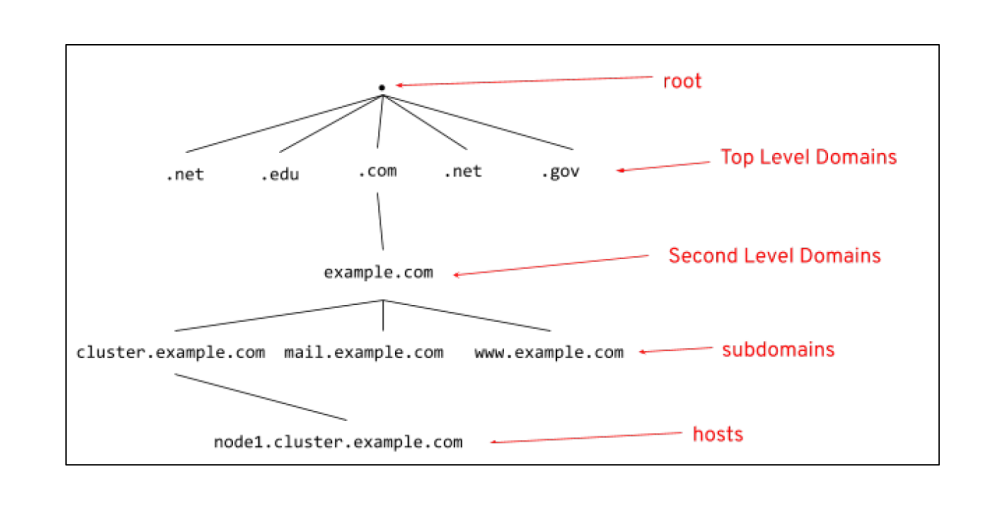
\includegraphics[width=.7\linewidth]{immagini/NET_11/dns_namespace.png}
    \caption{Struttura gerarchica del namespace DNS: dalla root ai Top Level Domain (TLD), ai domini di secondo livello, ai sottodomini e agli host finali.}
    \label{fig:dns_namespace}
\end{figure}

\subsection{Richiamo sul funzionamento del DNS}

\subsubsection{Modello client--server}
Il DNS adotta un modello client--server distribuito, in cui la risoluzione coinvolge diversi attori. Il client, tipicamente uno \emph{stub resolver} integrato nel sistema operativo o nell’applicazione, invia una query a un resolver ricorsivo configurato localmente (spesso fornito dall’ISP o dall’organizzazione).

Il \emph{recursive resolver} opera per conto del client: esegue le interrogazioni necessarie verso l’esterno, segue le deleghe nel namespace e mantiene una cache per riusare i risultati. I \emph{nameserver autoritativi} sono invece la fonte definitiva dei dati per una certa zona e rispondono con i record ufficiali pubblicati dall’amministratore della zona.

Un punto cruciale, anche in ottica di sicurezza, è che lo stub resolver si affida al resolver ricorsivo: se quest’ultimo accetta dati errati e li mette in cache, l’errore si propaga a tutti i client che lo utilizzano.

\subsubsection{Risoluzione ricorsiva}
Quando il resolver non dispone dell’informazione in cache, avvia una risoluzione che attraversa la gerarchia DNS. In generale, parte interrogando un server root per ottenere un riferimento ai server del TLD; poi contatta un server del TLD per ottenere i nameserver autoritativi del dominio; infine interroga il nameserver autoritativo per ottenere il record richiesto.

Le risposte DNS sono strutturate in sezioni. L’\emph{Answer section} contiene i record che rispondono direttamente alla query; l’\emph{Authority section} fornisce indicazioni sui nameserver autoritativi; l’\emph{Additional section} può includere record ausiliari (come i glue) utili a evitare query aggiuntive.

\begin{figure}[H]
    \centering
    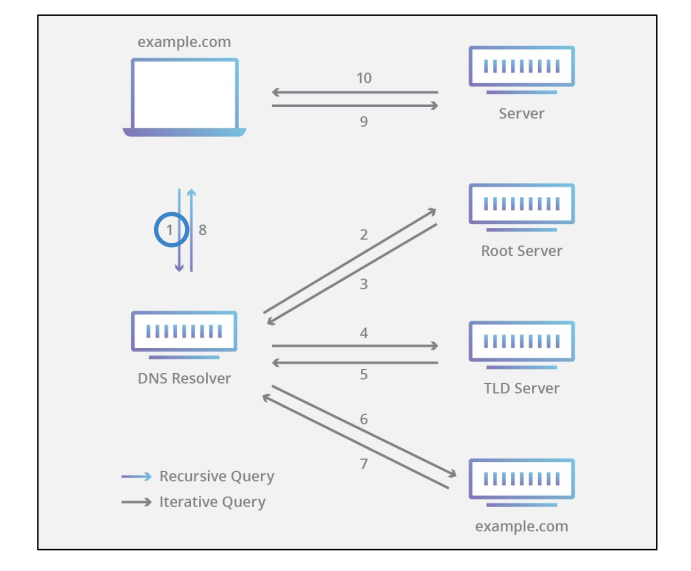
\includegraphics[width=.8\linewidth]{immagini/NET_11/resolution}
    \caption{Sequenza di risoluzione DNS: il client invia una query ricorsiva al resolver, che esegue query iterative verso root server, TLD server e nameserver autoritativo fino a ottenere il record richiesto. La risposta viene restituita al client e può essere memorizzata in cache secondo il TTL.}
    \label{fig:resolution}
\end{figure}

\subsubsection{Caching}
Il caching è un elemento chiave del DNS: riduce latenza e carico, perché evita di ripetere interrogazioni verso i nameserver autoritativi. La cache è tipicamente mantenuta dal resolver ricorsivo, ma può esistere anche a livello di browser e sistema operativo.

In cache possono finire record “positivi” (es. A/AAAA e NS) e record “negativi”, che attestano l’inesistenza di un nome (NXDOMAIN) o l’assenza di uno specifico tipo di record. Ogni entry è associata a un \textbf{TTL (Time To Live)}: finché il TTL non scade, il resolver può riusare la risposta senza nuove query.

Dal punto di vista della sicurezza, il caching è un moltiplicatore di impatto: se un resolver accetta un dato falso e lo memorizza, l’effetto dell’attacco persiste fino alla scadenza del TTL, influenzando molte risoluzioni successive.

\subsection{Vulnerabilità e attacchi noti sul DNS}

\subsubsection{Vulnerability 1: DNS spoofing e cache poisoning}
Con \textbf{DNS spoofing} (o \textbf{cache poisoning}) si indica l’inserimento di informazioni DNS false nella cache di un resolver, con l’obiettivo di far restituire al client un risultato errato (tipicamente un indirizzo IP controllato dall’attaccante). La conseguenza può essere la redirezione verso siti malevoli, il furto di credenziali, la distribuzione di malware o, più in generale, l’intercettazione/alterazione del traffico applicativo.

Un resolver non accetta però risposte arbitrarie: elabora solo risposte coerenti con una query pendente. In pratica, l’attaccante deve riuscire a produrre una risposta che “sembri” valida rispetto ai parametri della richiesta in corso (ad esempio identificatore della transazione e parametri di trasporto) e, soprattutto, deve farla arrivare prima della risposta legittima. Il comportamento del DNS segue infatti il principio operativo per cui la prima risposta considerata valida per una query pendente viene accettata, e le successive vengono scartate.

\begin{figure}[H]
    \centering
    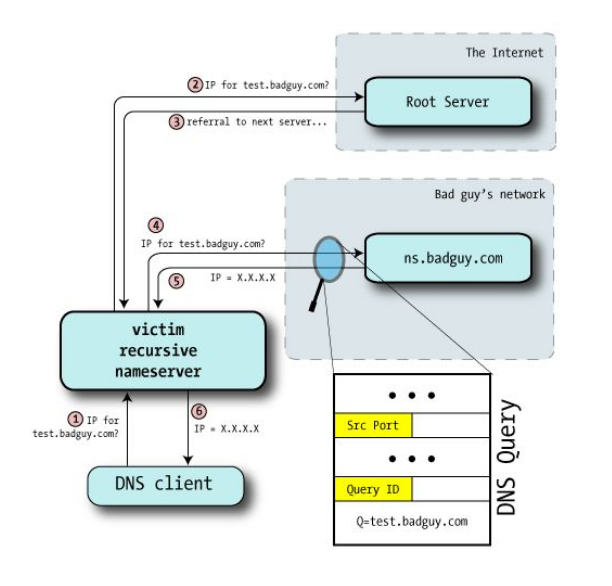
\includegraphics[width=.8\linewidth]{immagini/NET_11/queryid.png}
    \caption{Scenario di DNS spoofing: l’attaccante tenta di inviare una risposta falsa al resolver vittima durante la finestra in cui la query verso il nameserver autoritativo è pendente.}
    \label{fig:queryid}
\end{figure}

\subsubsection{Attacco di cache poisoning classico: dinamica e limiti}
Nel caso classico, l’attaccante induce (direttamente o indirettamente) una risoluzione per un nome non presente in cache, così da aprire una finestra temporale in cui la query è pendente. In quella finestra invia molte risposte forgiate con l’obiettivo di “indovinare” i parametri necessari all’accettazione. Se una risposta forged valida arriva prima di quella autentica, il resolver la accetta e memorizza i record; l’effetto persiste per il TTL.

Questo attacco è reso difficile dall’entropia dei parametri (ad esempio identificatori e porte) e dalla breve finestra temporale disponibile. Proprio per questo, le difese moderne puntano a introdurre un controllo crittografico dell’origine e dell’integrità dei dati (DNSSEC), così da rendere insufficiente la sola “coerenza” della risposta rispetto alla query pendente.

\begin{figure}[H]
    \centering
    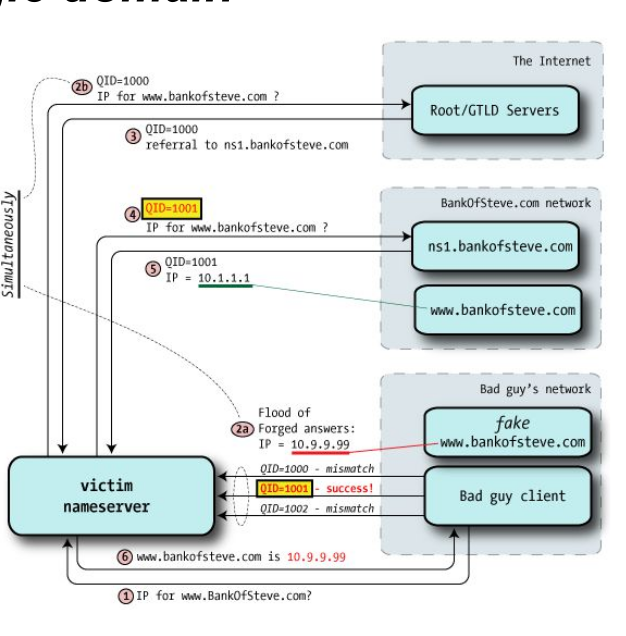
\includegraphics[width=.8\linewidth]{immagini/NET_11/cache_poisoning.png}
    \caption{Attacco di cache poisoning: durante una query DNS pendente, l’attaccante invia un flood di risposte forged; una risposta con parametri corretti viene accettata dal resolver e inserita in cache.}
    \label{fig:cache_poisoning}
\end{figure}

\subsubsection{Vulnerability 2: DNS tunneling}
Un abuso diverso del DNS consiste nell’utilizzarlo come canale di comunicazione “nascosto” per trasportare dati applicativi all’interno di query e risposte DNS, tecnica nota come \textbf{DNS tunneling}. In contesti reali, viene spesso sfruttata da malware e botnet per command-and-control o per esfiltrazione dati, perché il traffico DNS è comunemente consentito attraverso firewall e apparati di filtraggio.

L’idea è incapsulare dati nelle label del nome richiesto (query) e ricevere risposte che contengono payload o comandi all’interno di record DNS. La normalità apparente del traffico rende più complessa la distinzione tra uso legittimo e uso malevolo, soprattutto con controlli superficiali o basati solo su porte/protocolli.

\begin{figure}[H]
    \centering
    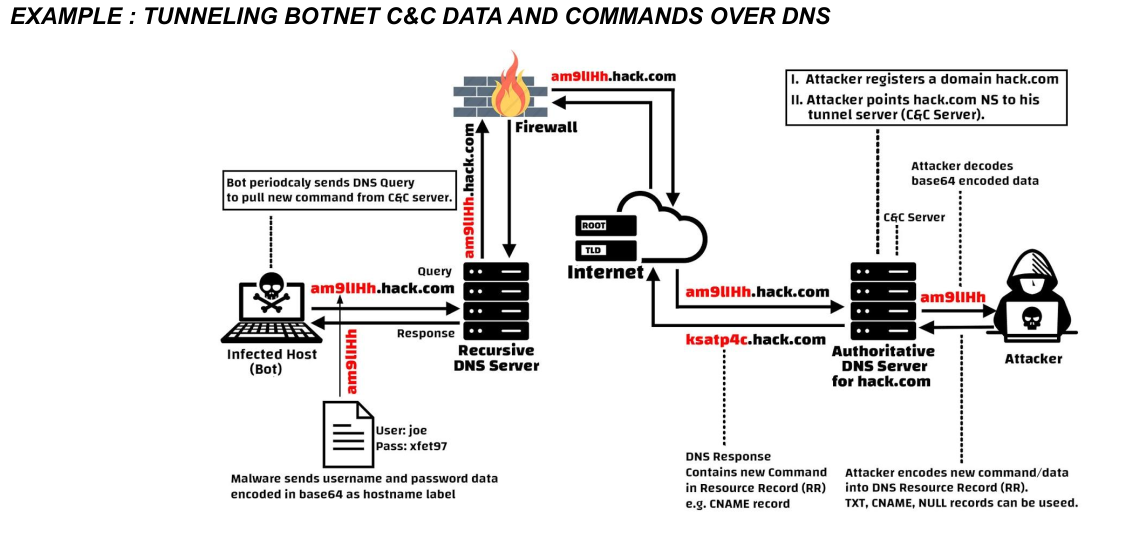
\includegraphics[width=.9\linewidth]{immagini/NET_11/dnsar}
    \caption{Esempio di DNS tunneling per command-and-control: dati e comandi vengono veicolati in query e risposte DNS, sfruttando il fatto che il DNS è spesso permesso in uscita/entrata dalle policy di rete.}
    \label{fig:dnsar}
\end{figure}

\subsubsection{Vulnerability 3: DNS hijacking}
Il \textbf{DNS hijacking} è il dirottamento delle risoluzioni verso infrastrutture controllate da un attaccante, senza necessariamente avvelenare la cache di un resolver. Può avvenire a livello di configurazione (ad esempio modificando i DNS configurati su un host o su un router), a livello di rete (attacchi man-in-the-middle) o a livello di gestione del dominio (compromissione dell’account presso il provider/registrar, con modifica dei record).

DNSSEC può ridurre l’impatto del hijacking solo se lungo il percorso di risoluzione viene effettivamente eseguita la validazione DNSSEC e la catena di fiducia è integra. In assenza di validazione, o se l’attacco riesce a imporre un resolver che non valida, l’utente può essere comunque reindirizzato verso risposte non affidabili.

\subsubsection{Vulnerability 4: NXDOMAIN attack}
Tra gli attacchi orientati alla disponibilità rientrano i \textbf{NXDOMAIN attack}, in cui un attaccante inonda un server DNS (autoritativo o ricorsivo) con richieste per nomi inesistenti. Se le richieste sono costruite in modo da evitare il caching (ad esempio generando sottodomini casuali), il server è costretto a elaborare un elevato numero di miss, consumando risorse e degradando il servizio per il traffico legittimo. Varianti note includono attacchi a sottodomini random o “phantom domain”.

\subsubsection{Vulnerability 5: confidenzialità delle query DNS}
Un problema strutturale del DNS tradizionale è la mancanza di \textbf{confidenzialità}: query e risposte viaggiano in chiaro. Questo permette a osservatori on-path (provider, amministratori di rete, attaccanti passivi) di inferire siti e servizi utilizzati, con impatti su privacy e, in alcuni scenari, su sicurezza e libertà di accesso (ad esempio attraverso forme di censura o profilazione).

DNSSEC non risolve questo problema: autentica i dati, ma non cifra il canale. Per la privacy del canale sono necessari protocolli dedicati, come DNS over TLS e DNS over HTTPS (discussioni più avanti).

\subsection{DNSSEC: motivazioni, obiettivi e principio di funzionamento}

\subsubsection{Perché DNSSEC}
Il DNS tradizionale non consente al resolver di verificare crittograficamente l’origine dei dati né la loro integrità. Questo rende possibili attacchi in cui l’attaccante introduce informazioni false (in particolare cache poisoning) o altera risposte in transito. DNSSEC (\emph{Domain Name System Security Extensions}) nasce per introdurre meccanismi che permettono di verificare che i dati provengano dalla zona autoritativa corretta e che non siano stati modificati.

È importante chiarire lo \emph{scope}: DNSSEC mira a garantire \textbf{integrità} e \textbf{autenticità} dei dati DNS e a supportare una \textbf{negazione autenticata dell’esistenza} (dimostrare in modo firmato che un nome o un record non esiste). Non fornisce invece confidenzialità delle query e non impedisce attacchi DoS; anzi, l’aumento della dimensione delle risposte può influenzare scenari di amplification.

\subsubsection{RRset e firme}
DNSSEC introduce la firma digitale dei dati DNS. Nel DNS, le informazioni sono espresse come \emph{Resource Record} (RR) e, in DNSSEC, non si firma il singolo record isolato, ma un insieme coerente di record con stesso nome, tipo e classe, detto \emph{RRset}. La firma di un RRset viene pubblicata in un record dedicato, \textbf{RRSIG}. Un resolver considera un RRset affidabile solo se la verifica della firma ha successo.

\subsubsection{DNSKEY, ZSK e KSK}
Una zona firmata pubblica chiavi pubbliche tramite record \textbf{DNSKEY}. Operativamente si distinguono due ruoli:
\begin{itemize}
    \item \textbf{ZSK} (\emph{Zone Signing Key}), usata per firmare gli RRset “operativi” della zona;
    \item \textbf{KSK} (\emph{Key Signing Key}), usata per firmare l’RRset DNSKEY, cioè per attestare quali chiavi pubbliche sono valide per la zona.
\end{itemize}
Questa separazione facilita la gestione dei cambi chiave (\emph{key rollover}): la rotazione della ZSK è in genere più semplice, mentre la rotazione della KSK impatta anche la relazione con la zona padre.

\begin{figure}[H]
    \centering
    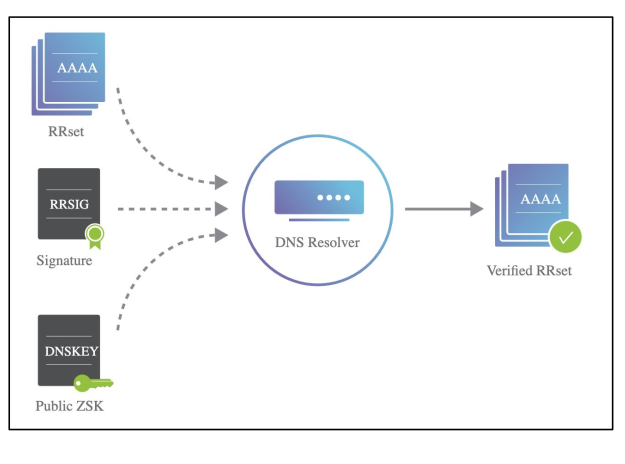
\includegraphics[width=.8\linewidth]{immagini/NET_11/zsk.png}
    \caption{Verifica DNSSEC di un RRset: il resolver controlla la firma RRSIG utilizzando la chiave pubblica ZSK pubblicata nel record DNSKEY, ottenendo un RRset verificato.}
    \label{fig:zsk}
\end{figure}

\subsubsection{DS e catena di fiducia}
Per estendere la fiducia lungo la gerarchia DNS, DNSSEC introduce il record \textbf{DS} (\emph{Delegation Signer}). Il DS è pubblicato nella zona padre e contiene un digest (hash) della KSK della zona figlia. Quando il resolver ottiene i DNSKEY della zona figlia, calcola il digest della KSK e lo confronta con il DS ottenuto dal padre: se coincidono, il resolver può ritenere autentica la KSK della figlia e usarla per validare le firme all’interno della zona.

Ripetendo questo meccanismo lungo la gerarchia, si ottiene una \textbf{catena di fiducia} (\emph{chain of trust}) che, idealmente, risale fino alla root.

\begin{figure}[H]
    \centering
    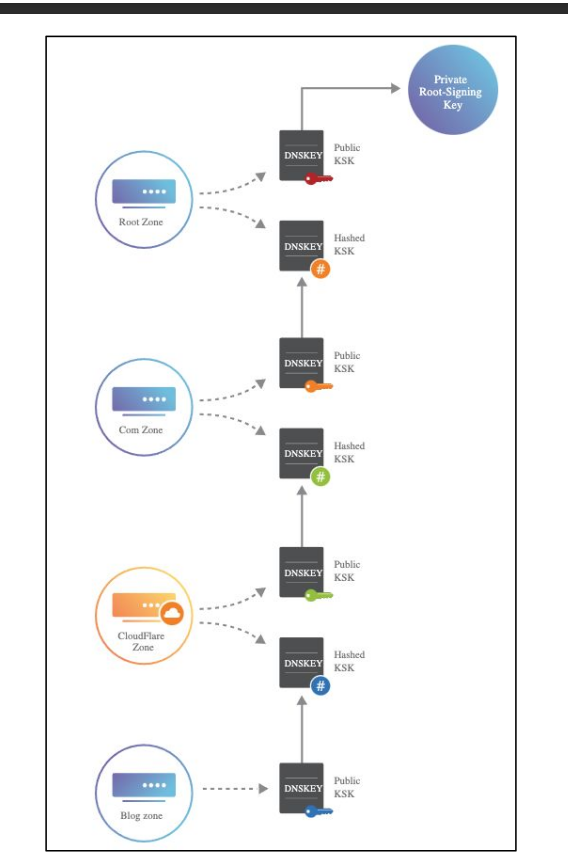
\includegraphics[width=.65\linewidth]{immagini/NET_11/chain.png}
    \caption{Catena di fiducia DNSSEC: ogni zona padre autentica la zona figlia tramite DS (digest della KSK), consentendo al resolver di validare progressivamente i dati fino alla zona finale.}
    \label{fig:chain}
\end{figure}

\subsubsection{Trust anchor e stati di validazione}
La validazione DNSSEC richiede un \emph{trust anchor}, ossia una chiave pubblica considerata affidabile a priori (tipicamente la root). In base agli esiti delle verifiche, un resolver classifica le risposte come:
\begin{itemize}
    \item \emph{secure}: firma e catena di fiducia valide;
    \item \emph{insecure}: la zona non è firmata (o non è collegata alla catena) ma la situazione è coerente con una delega non-DNSSEC;
    \item \emph{bogus}: la validazione fallisce (firme non verificabili, DS incoerenti, catena interrotta in modo non giustificabile).
\end{itemize}
Le risposte \emph{bogus} vengono scartate perché non affidabili.

\subsection{Negazione autenticata e rischio di zone enumeration}

\subsubsection{NSEC e “zone walking”}
DNSSEC deve poter dimostrare in modo firmato anche la non-esistenza di un nome o di un tipo di record. Un semplice \texttt{NXDOMAIN} non firmato non sarebbe sufficiente, perché un attaccante potrebbe falsificarlo. Per questo vengono introdotti record di negazione autenticata come \textbf{NSEC}.

NSEC funziona collegando logicamente i nomi esistenti in una zona in un ordine (lessicografico): per dimostrare che un certo nome non esiste, si restituisce un NSEC che copre l’intervallo in cui quel nome “cadrebbe”, e il record è firmato. Il prezzo di questa soluzione è informativo: seguendo i puntatori “next”, un attaccante può effettuare \textbf{zone walking} e ricostruire l’elenco dei nomi presenti nella zona.

\subsubsection{NSEC3 e attacchi a dizionario}
Per ridurre la facilità di enumerazione, \textbf{NSEC3} sostituisce i nomi in chiaro con hash (con salt). In questo modo, i puntatori non rivelano direttamente i nomi. Tuttavia, l’informazione non scompare: un attaccante può tentare un \textbf{dictionary attack} calcolando hash di candidate label e verificando se compaiono nella zona. In pratica, la “privacy” dei sottodomini dipende da quanto sono difficili da indovinare.

\subsection{DNSSEC white lies}

\subsubsection{Idea generale}
Per mitigare l’enumerazione con NSEC, è possibile adottare una tecnica nota come \textbf{DNSSEC white lies}. L’obiettivo è continuare a fornire una negazione autenticata corretta (quindi verificabile dal resolver), evitando però di rivelare in modo sistematico “il prossimo nome reale” nella catena NSEC.

Operativamente, il nameserver autoritativo può produrre NSEC “plausibili” che dimostrano la non-esistenza del \emph{QNAME} richiesto, ma non costituiscono un puntatore affidabile per camminare l’intera zona. Questo implica tipicamente la \textbf{generazione e firma on-demand} di NSEC costruiti ad hoc per la query.

\subsubsection{Considerazioni di sicurezza e operative}
L’adozione delle white lies introduce costi e rischi non trascurabili. Se il server deve firmare al volo, deve avere accesso alle chiavi private su macchine esposte in rete, aumentando la superficie di rischio. Inoltre, la firma digitale è più costosa di una risposta DNS “statica”: un attaccante può forzare molte richieste verso nomi inesistenti per indurre lavoro crittografico e causare denial of service. Infine, la robustezza della tecnica dipende anche dalla qualità e imprevedibilità delle scelte con cui vengono generati i nomi “fittizi” utilizzati nei record prodotti dinamicamente.

\subsection{DNSSEC e minaccia Reflection/Amplification}

\subsubsection{Perché DNSSEC aumenta l’amplification potenziale}
DNS (e DNSSEC) opera spesso su UDP: questo rende possibile lo spoofing dell’indirizzo sorgente e abilita attacchi di \emph{reflection}. DNSSEC tende inoltre ad aumentare la dimensione delle risposte, perché oltre ai record richiesti possono essere restituiti anche RRSIG e, in alcuni casi, chiavi DNSKEY necessarie alla validazione. Ne deriva che query relativamente piccole possono generare risposte molto più grandi, aumentando il fattore di amplificazione.

\subsubsection{Ordini di grandezza}
In scenari tipici, risposte firmate per query negative possono essere molte volte più grandi delle corrispondenti risposte non firmate. Inoltre, alcune query particolarmente “ricche” (storicamente, la \texttt{ANY}) possono produrre risposte ancora più voluminose, rendendo l’infrastruttura DNS un target appetibile per attacchi DDoS basati su reflection/amplification.

\subsection{ECDSA in DNSSEC: motivazioni e benefici}

\subsubsection{Firma più efficiente e risposte più piccole}
L’impiego di algoritmi come \textbf{ECDSA} in DNSSEC è motivato da due esigenze operative: rendere più sostenibile la firma on-demand (utile, ad esempio, per tecniche come le white lies) e ridurre la dimensione delle risposte firmate. A parità di livello di sicurezza, ECDSA utilizza chiavi e firme significativamente più piccole rispetto a RSA, con impatto diretto sul payload DNSSEC e, quindi, sull’amplification potenziale.

\subsubsection{Impatto sull’adozione}
In una prospettiva di deployment, la combinazione di firme più veloci e dimensioni inferiori può abbassare due barriere pratiche: la gestione del rischio di enumerazione (quando si punta a negazioni autenticare senza esporre troppo la zona) e la riduzione del contributo di DNSSEC agli scenari di amplification. Resta comunque fondamentale considerare che la sicurezza del DNS non dipende da un singolo meccanismo: DNSSEC risolve autenticità e integrità, ma non copre la confidenzialità del canale né i problemi di disponibilità.

\subsection{Perché DNSSEC non basta: DNS over TLS (DoT) e DNS over HTTPS (DoH)}

\subsubsection{Limite strutturale: assenza di confidenzialità}
DNSSEC protegge i dati DNS (integrità/autenticità), ma non cifra le query. Se l’obiettivo è impedire l’osservazione del traffico DNS in transito, sono necessari protocolli che cifrano il canale tra client e resolver.

\subsubsection{DNS over TLS (DoT)}
DoT incapsula DNS in una sessione TLS su TCP. Il client stabilisce una connessione TCP verso un server DoT e completa l’handshake TLS; successivamente scambia messaggi DNS all’interno del canale cifrato. Per motivi prestazionali, è importante riutilizzare la connessione e, quando possibile, inviare più query nella stessa sessione, così da ammortizzare i costi di setup TCP/TLS.

\subsubsection{DNS over HTTPS (DoH)}
DoH trasporta query e risposte DNS come scambi HTTP(S). Ogni query può essere mappata in una richiesta HTTP (GET o POST), e la protezione deriva dall’uso di TLS a livello HTTPS. Dal punto di vista di rete, DoH tende a confondersi con traffico web standard: questo può aumentare la privacy dell’utente, ma riduce la capacità di alcune organizzazioni di applicare policy e monitoraggio DNS a livello di rete senza intervenire in modo più invasivo.

\subsubsection{DoT vs DoH: trade-off}
DoT è spesso più distinguibile e quindi più “gestibile” in ambito enterprise (porta dedicata e traffico identificabile), mentre DoH, essendo incapsulato in HTTPS, è più difficile da filtrare selettivamente senza impattare il traffico web in generale. In pratica, la scelta riflette un compromesso tra esigenze di controllo amministrativo e obiettivi di privacy.


\subsection{Lab: abilitazione DNSSEC con BIND (procedura e significato)}

\subsubsection{Obiettivo del laboratorio}
Nel laboratorio l’obiettivo è firmare una zona (ad esempio \texttt{angelotulumello.xyz}) e pubblicarla con BIND, completando poi la catena di fiducia pubblicando il record DS presso il registrar. Senza questo passo, la zona rimane firmata localmente ma non risulta validabile come \emph{secure} da resolver esterni: è una tipica \emph{island of security}.

\subsubsection{Passi essenziali: chiavi, firma e pubblicazione}
A livello operativo, la procedura si articola in tre momenti: (i) generazione di ZSK e KSK, (ii) inclusione delle DNSKEY pubbliche nella zona e firma della zona (ottenendo il file \texttt{.signed} e il \texttt{dsset-<zona>}), (iii) configurazione di BIND per servire la zona firmata e caricamento del DS nel pannello del registrar, così che il parent certifichi la delega.

Il punto concettuale del laboratorio è che DNSSEC non è “solo firme nella zona”: la proprietà di essere \emph{secure} dipende dall’intera catena, quindi dalla corretta pubblicazione del DS nel parent e dalla validazione lato resolver.
